\documentclass[12pt,ngerman,parkskip=half]{scrreprt}
\usepackage{babel} % Alternative: polyglossia
\usepackage{blindtext} % für Dummy Text
\usepackage{graphicx} % Bilder einbinden
\usepackage{booktabs} % schöne Tabellen


\title{Mein Wiederholungsdokument}
\author{Uwe Ziegenhagen}

\begin{document}
\maketitle

\tableofcontents

\listoffigures

\listoftables

\chapter{Einleitung}

\section{Literatur}

\subsection{vor 1900}

\subsubsection{Europa}

\blindtext[3]

\begin{figure}[h]
\begin{center}
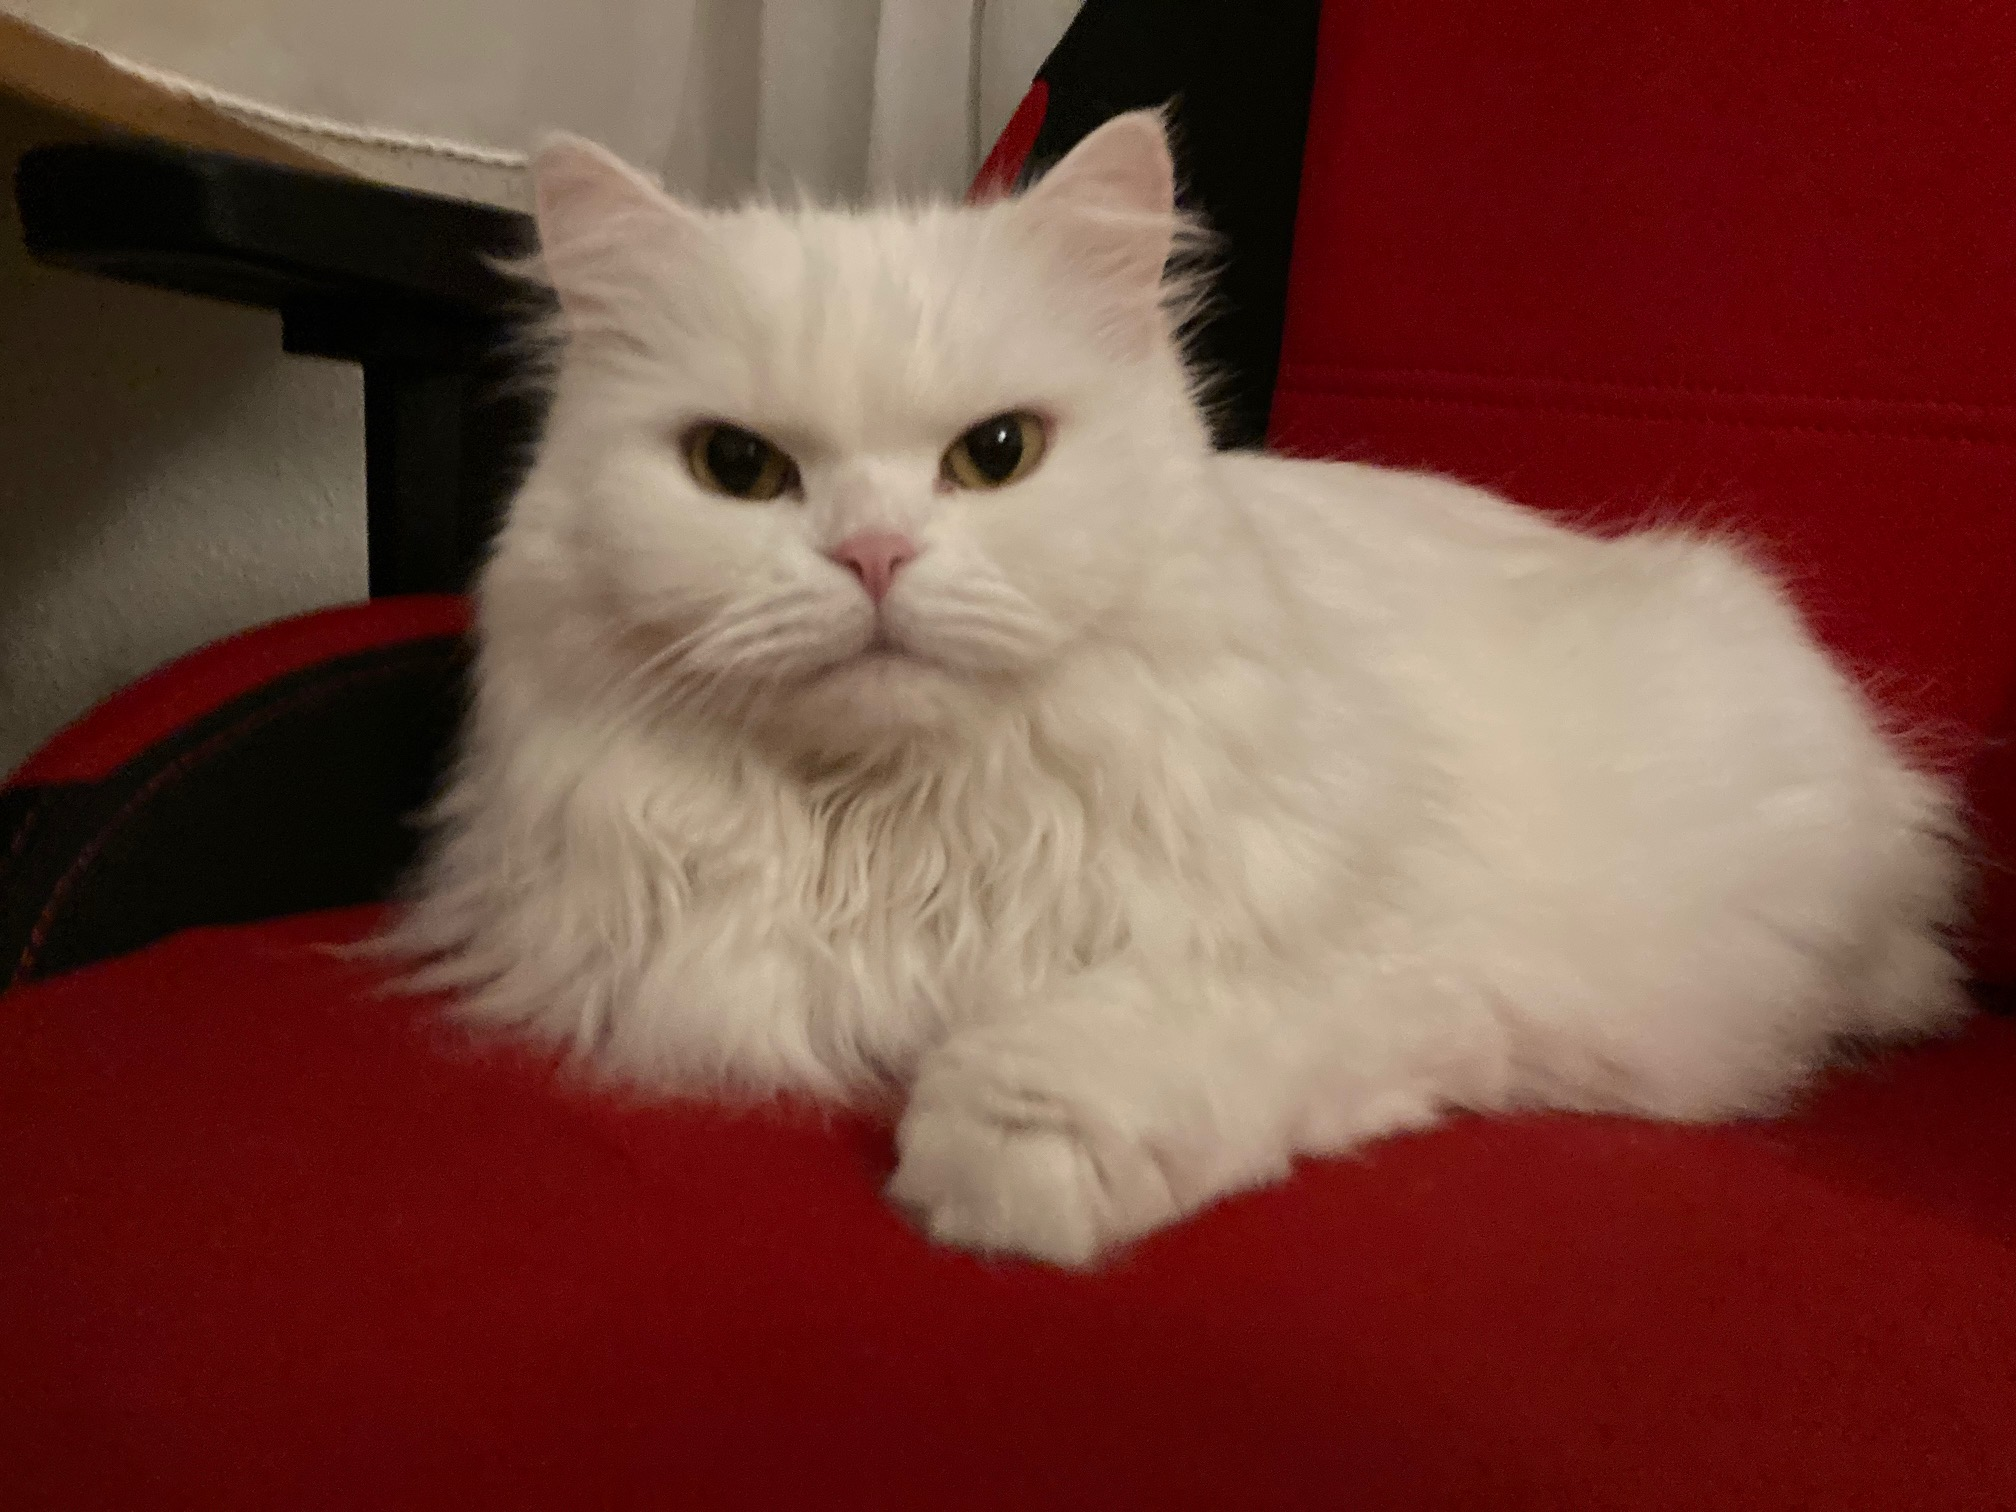
\includegraphics[width=0.9\textwidth]{Bilder/Katze}
\caption{Melli - der kleine Teufel}\label{fig:Katze}
\end{center}
\end{figure}

\blindtext[3]

\blindtext

\chapter[Kernanalyse der eurozentristischen Kunstpolitik]{Kernanalyse der eurozentristischen Kunstpolitik im Europa des 19. Jahrhunderts im Vergleich zwischen Eisenhower und Stalin}

\begin{table}
\begin{center}
\caption{Meine einzige Tabelle}\label{tab:tabelle}
\begin{tabular}{lrcp{6cm}} \toprule 
Spalte 1 & Spalte 2 & Spalte 3 & Spalte 4 \\ \midrule
52435 & 543253 & 534 3244 & Hallo Welt, ich bin ein Text \\
55 & 553 & 533244 & Hallo Welt, ich bin ein Text im Dokument\\ \bottomrule
\end{tabular}
\end{center}
\end{table}


\begin{tabular}{llllll}
0,826802253	&	0,673081547	&	0,728854475	&	0,557510822	&	0,092072115	&	0,776507665	\\
0,350192427	&	0,830353062	&	0,843233104	&	0,864630384	&	0,321438039	&	0,111815129	\\
0,047859381	&	0,225824054	&	0,473902663	&	0,677181476	&	0,114812073	&	0,242458895	\\
0,438051968	&	0,040396679	&	0,633195519	&	0,631907775	&	0,025947965	&	0,259953143	\\
0,450243312	&	0,285852868	&	0,728264867	&	0,513597795	&	0,185996715	&	0,258570467	\\
0,78520927	&	0,975260276	&	0,165080938	&	0,513674956	&	0,779636013	&	0,96725494	\\
0,135971402	&	0,864882366	&	0,13515706	&	0,619963022	&	0,870139315	&	0,725932946	\\
0,15144127	&	0,556541221	&	0,226173056	&	0,9442022	&	0,785742584	&	0,38123488	\\
0,469153038	&	0,37889537	&	0,831327685	&	0,058552755	&	0,834415014	&	0,120718184	\\
0,210250682	&	0,70637068	&	0,818163203	&	0,426081674	&	0,83118347	&	0,625251883	\\
0,700210488	&	0,742677688	&	0,570321107	&	0,274557587	&	0,821501129	&	0,088493387	\\
0,031902232	&	0,106768727	&	0,96127706	&	0,980532339	&	0,958298759	&	0,180713875	\\
0,829146495	&	0,465202602	&	0,785096301	&	0,085250785	&	0,332163514	&	0,30806315	\\
0,085108722	&	0,13356567	&	0,863159727	&	0,499259235	&	0,664616856	&	0,884915828	\\
0,589478771	&	0,211783365	&	0,705335457	&	0,175148788	&	0,634578374	&	0,771512014	\\
0,606451785	&	0,354610225	&	0,011033282	&	0,812408115	&	0,695319889	&	0,734536931	\\
0,462361092	&	0,72019136	&	0,412203264	&	0,133707107	&	0,011367899	&	0,964286547	\\
0,403354228	&	0,15346209	&	0,598369538	&	0,411971657	&	0,353859333	&	0,28979193	\\
0,669120848	&	0,215040211	&	0,984888825	&	0,273311259	&	0,999584832	&	0,709726027	\\
0,244327455	&	0,273713695	&	0,61224926	&	0,186143367	&	0,634134317	&	0,358937151	\\
0,68810667	&	0,638564019	&	0,423664769	&	0,000880311	&	0,348707817	&	0,487199559	\\
0,774974309	&	0,968375773	&	0,615318194	&	0,628956115	&	0,256361416	&	0,567851334	\\
0,358218569	&	0,250770708	&	0,818260571	&	0,748089415	&	0,948533088	&	0,450007136	\\
0,453262274	&	0,859299752	&	0,055536016	&	0,225181618	&	0,769367391	&	0,582758152	\\
0,426996431	&	0,254677587	&	0,685278311	&	0,768225563	&	0,322123755	&	0,054583524	\\
0,388667674	&	0,126170335	&	0,966518185	&	0,758486758	&	0,772861939	&	0,030618366	\\
0,112482489	&	0,434830193	&	0,639030944	&	0,167040395	&	0,086547116	&	0,779291336	\\
0,220377384	&	0,023652804	&	0,568398995	&	0,776444318	&	0,222337626	&	0,324777109	\\
0,10705612	&	0,666858134	&	0,796002848	&	0,170704357	&	0,510981001	&	0,766787983	\\
0,692469228	&	0,785892688	&	0,08611552	&	0,930894215	&	0,544888912	&	0,377205498	\\
0,386175267	&	0,438791933	&	0,882485072	&	0,580653132	&	0,486919155	&	0,574240857	\\
\end{tabular}




\end{document}